% Q5V2: Wi-Fi through wall — Signal path diagram
% AP → concrete wall → air → laptop
\documentclass[border=10pt]{standalone}
\usepackage{tikz}
\usepackage{amsmath}
\usetikzlibrary{arrows.meta, decorations.pathreplacing}
\renewcommand{\familydefault}{\sfdefault}

\begin{document}
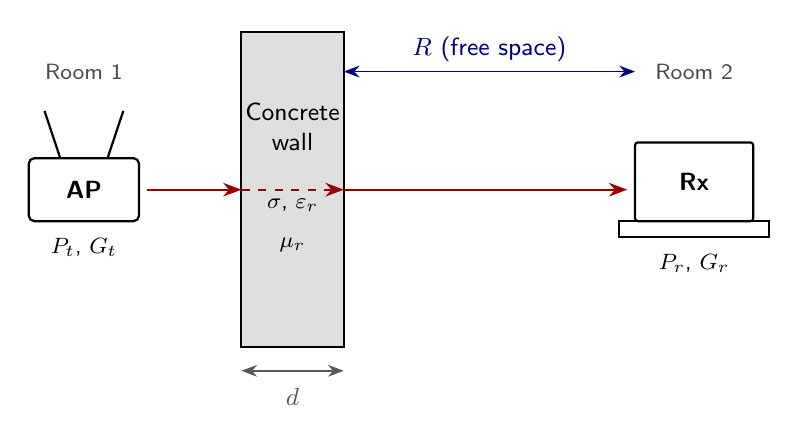
\begin{tikzpicture}[
    every node/.style={font=\sffamily},
    >=Stealth,
]

% === Concrete wall ===
\fill[gray!25, draw=black, line width=0.8pt]
    (3.5,0) rectangle (4.8,4);
\node[font=\sffamily\small, align=center] at (4.15, 2.8) {Concrete\\wall};
\node[font=\sffamily\footnotesize] at (4.15, 1.8) {$\sigma$, $\varepsilon_r$};
\node[font=\sffamily\footnotesize] at (4.15, 1.3) {$\mu_r$};

% === Wall thickness dimension ===
\draw[<->, line width=0.6pt, gray!70!black] (3.5, -0.3) -- (4.8, -0.3);
\node[below, font=\sffamily\small, gray!70!black] at (4.15, -0.4) {$d$};

% === Wi-Fi AP (transmitter, left side) ===
% Router icon
\draw[thick, rounded corners=2pt] (0.8, 1.6) rectangle (2.2, 2.4);
\draw[thick] (1.2, 2.4) -- (1.0, 3.0);
\draw[thick] (1.8, 2.4) -- (2.0, 3.0);
\node[font=\sffamily\small\bfseries] at (1.5, 2.0) {AP};
\node[below, font=\sffamily\footnotesize] at (1.5, 1.5) {$P_t$, $G_t$};

% === Laptop (receiver, right side) ===
% Laptop icon
\draw[thick, rounded corners=1pt] (8.5, 1.6) rectangle (10.0, 2.6);
\draw[thick] (8.3, 1.4) -- (8.3, 1.6) -- (10.2, 1.6) -- (10.2, 1.4) -- cycle;
\node[font=\sffamily\small\bfseries] at (9.25, 2.1) {Rx};
\node[below, font=\sffamily\footnotesize] at (9.25, 1.3) {$P_r$, $G_r$};

% === Signal path arrow ===
\draw[->, thick, red!60!black] (2.3, 2.0) -- (3.5, 2.0);
\draw[->, thick, red!60!black, dashed] (3.5, 2.0) -- (4.8, 2.0);
\draw[->, thick, red!60!black] (4.8, 2.0) -- (8.4, 2.0);

% === Free-space path dimension ===
\draw[<->, line width=0.6pt, blue!50!black] (4.8, 3.5) -- (8.5, 3.5);
\node[above, font=\sffamily\small, blue!50!black] at (6.65, 3.5) {$R$ (free space)};

% === Room labels ===
\node[font=\sffamily\footnotesize, gray!60!black] at (1.5, 3.5) {Room 1};
\node[font=\sffamily\footnotesize, gray!60!black] at (9.25, 3.5) {Room 2};

\end{tikzpicture}
\end{document}
